\documentclass[12pt,a4paper]{article}

% ─── Page Layout ───────────────────────────────────────────────────────────────
\usepackage[a4paper, margin=0.8in, headheight=14pt]{geometry}

% ─── Fonts (XeLaTeX) ───────────────────────────────────────────────────────────
\usepackage{fontspec}
\usepackage{unicode-math}
\setmainfont{TeX Gyre Pagella}
\setmonofont[Scale=0.88]{TeX Gyre Cursor}
\setmathfont{Latin Modern Math}

% ─── Packages ──────────────────────────────────────────────────────────────────
\usepackage{xcolor}
\usepackage{colortbl}
\usepackage{titlesec}
\usepackage{enumitem}
\usepackage{tabularx}
\usepackage{booktabs}
\usepackage{array}
\usepackage{amsmath}
\usepackage{tikz}
\usetikzlibrary{shapes.geometric, arrows.meta, positioning, calc, fit, decorations.pathreplacing}
\usepackage{tcolorbox}
\tcbuselibrary{skins, breakable}
\usepackage{hyperref}
\usepackage{fancyhdr}
\usepackage{graphicx}
\usepackage{microtype}
\hyphenpenalty=10000
\exhyphenpenalty=10000
\sloppy
\usepackage{caption}
\usepackage{setspace}
\usepackage{multirow}
\usepackage{tocloft}

% ─── Q&A helper ────────────────────────────────────────────────────────────────
\newcommand{\Q}[1]{\textbf{#1}\par\noindent\ignorespaces}

% ─── Colour Palette ────────────────────────────────────────────────────────────
\definecolor{myred}{RGB}{196,30,58}
\definecolor{mydark}{RGB}{30,30,50}
\definecolor{mygreen}{RGB}{14,120,80}
\definecolor{myteal}{RGB}{0,130,140}
\definecolor{myamber}{RGB}{180,100,0}
\definecolor{mypurple}{RGB}{100,30,160}
\definecolor{mygray}{RGB}{246,247,249}
\definecolor{mgframe}{RGB}{180,185,200}
\definecolor{watermark}{RGB}{145,150,170}
\definecolor{hdrred}{RGB}{250,232,235}
\definecolor{hdrgreen}{RGB}{220,244,233}
\definecolor{hdrteal}{RGB}{220,242,244}
\definecolor{hdramber}{RGB}{253,242,215}
\definecolor{hdrpurple}{RGB}{238,228,255}
\definecolor{hdrgray}{RGB}{238,240,245}
\definecolor{rowalt}{RGB}{250,251,253}

% ─── Section Formatting ────────────────────────────────────────────────────────
\titleformat{\section}{\large\bfseries\color{myred}}{\thesection.}{0.5em}{}[\vspace{1pt}{\color{myred}\rule{\linewidth}{0.8pt}}]
\titleformat{\subsection}{\normalsize\bfseries\color{myteal}}{\thesubsection}{0.5em}{}
\titlespacing*{\section}{0pt}{18pt}{7pt}
\titlespacing*{\subsection}{0pt}{11pt}{4pt}

% ─── Paragraph ─────────────────────────────────────────────────────────────────
\setlength{\parindent}{0pt}
\setlength{\parskip}{4pt}

% ─── TOC Styling ───────────────────────────────────────────────────────────────
\renewcommand{\cfttoctitlefont}{\large\bfseries\color{myred}}
\renewcommand{\cftaftertoctitle}{\par\noindent{\color{myred}\rule{\linewidth}{0.8pt}}}
\setlength{\cftbeforetoctitleskip}{0pt}
\setlength{\cftaftertoctitleskip}{6pt}
\renewcommand{\cftsecfont}{\normalsize\bfseries\color{mydark}}
\renewcommand{\cftsecpagefont}{\normalsize\bfseries\color{mydark}}
\renewcommand{\cftsecleader}{\cftdotfill{\cftdotsep}}
\setlength{\cftbeforesecskip}{7pt}
\renewcommand{\cftsubsecfont}{\small\color{mydark}}
\renewcommand{\cftsubsecpagefont}{\small\color{mydark}}
\setlength{\cftbeforesubsecskip}{3pt}
\setlength{\cftsubsecindent}{1.4em}

% ─── Table helpers ─────────────────────────────────────────────────────────────
\renewcommand{\arraystretch}{1.45}
\setlength{\tabcolsep}{6pt}
\arrayrulecolor{mydark}
\newcolumntype{B}[1]{>{\small\bfseries\raggedright\arraybackslash}m{#1}}
\newcolumntype{Y}{>{\small\raggedright\arraybackslash}X}
\renewcommand{\tabularxcolumn}[1]{m{#1}}

% ─── Header / Footer ───────────────────────────────────────────────────────────
\pagestyle{fancy}
\fancyhf{}
\fancyhead[L]{\small\color{myred}\textbf{PE-EC801B}\;\color{mydark}--- Fiber Optic Communication}
\fancyhead[R]{\small\color{myteal}\textbf{Module 1 Notes}}
\fancyfoot[C]{\small\color{mydark}\thepage}
\fancyfoot[R]{\small\color{watermark}\textit{\copyright\ Biraj}}
\renewcommand{\headrulewidth}{0.5pt}
\renewcommand{\footrulewidth}{0.3pt}

% ─── Hyperref ──────────────────────────────────────────────────────────────────
\hypersetup{colorlinks=true, linkcolor=myteal, urlcolor=myteal,
  pdfauthor={Biraj Sarkar}, pdftitle={PE-EC801B --- Module 1 Notes}}

% ─── tcolorbox styles ──────────────────────────────────────────────────────────
\tcbset{
  tikzbox/.style={colback=mygray, colframe=mgframe, boxrule=0.6pt, arc=4pt,
    left=8pt, right=8pt, top=6pt, bottom=6pt,
    colbacktitle=mgframe, coltitle=mydark, fonttitle=\small\bfseries},
  defbox/.style={colback=hdrgreen, colframe=mygreen, boxrule=0.8pt, arc=4pt,
    left=9pt, right=9pt, top=6pt, bottom=6pt,
    colbacktitle=mygreen, coltitle=white, fonttitle=\small\bfseries},
  formulabox/.style={colback=hdrteal, colframe=myteal, boxrule=0.8pt, arc=4pt,
    left=9pt, right=9pt, top=7pt, bottom=7pt,
    colbacktitle=myteal, coltitle=white, fonttitle=\small\bfseries},
  examplebox/.style={colback=hdramber, colframe=myamber, boxrule=0.8pt, arc=4pt,
    left=9pt, right=9pt, top=6pt, bottom=6pt,
    colbacktitle=myamber, coltitle=white, fonttitle=\small\bfseries},
  masonbox/.style={colback=hdrpurple, colframe=mypurple, boxrule=0.8pt, arc=4pt,
    left=9pt, right=9pt, top=6pt, bottom=6pt,
    colbacktitle=mypurple, coltitle=white, fonttitle=\small\bfseries},
  exambox/.style={colback=hdrpurple, colframe=mypurple, boxrule=1pt, arc=5pt,
    left=10pt, right=10pt, top=8pt, bottom=8pt,
    colbacktitle=mypurple, coltitle=white, fonttitle=\bfseries,
    breakable, title after break={\textbf{Frequently Asked / Viva Questions (contd.)}}}
}
\tcbset{breakable}

% ─── TikZ styles ───────────────────────────────────────────────────────────────
\tikzset{
  block/.style={rectangle, draw=myteal, fill=hdrteal,
    text width=2.4cm, align=center, minimum height=0.95cm,
    font=\small, rounded corners=3pt, line width=0.7pt},
  redblock/.style={rectangle, draw=myred, fill=hdrred,
    text width=2.4cm, align=center, minimum height=0.95cm,
    font=\small, rounded corners=3pt, line width=0.7pt},
  netnode/.style={rectangle, draw=myteal, fill=hdrteal,
    text width=1.5cm, align=center, minimum height=0.8cm,
    font=\small, rounded corners=3pt, line width=0.7pt},
  sumjunc/.style={circle, draw=myamber, fill=hdramber,
    minimum size=0.62cm, font=\small, line width=0.8pt},
  snode/.style={circle, draw=mypurple, fill=hdrpurple,
    minimum size=0.55cm, font=\footnotesize, line width=0.7pt},
  arrow/.style={-Stealth, thick, color=mydark},
  redarrow/.style={-Stealth, thick, color=myred},
  line/.style={thick, color=mydark}
}

% ═══════════════════════════════════════════════════════════════════════════════
\begin{document}
% ═══════════════════════════════════════════════════════════════════════════════

\begin{center}
  {\LARGE\bfseries\color{myred} PE-EC801B --- Fiber Optic Communication}\\[5pt]
  {\normalsize\color{mydark} Semester VIII \quad$\bullet$\quad 3L:0T:0P \quad$\bullet$\quad 3 Credits}\\[3pt]
  {\normalsize\color{myteal}\textbf{Module 1 Exam Notes}}\\[3pt]
  {\small\color{mydark} CGEC \;$|$\; B.Tech ECE (2023--27) \;$|$\; \textit{Biraj Sarkar}}
\end{center}
\vspace{2pt}
\noindent{\color{myred}\rule{\linewidth}{1.5pt}}
\vspace{2pt}

\hypersetup{linkcolor=mydark}
\tableofcontents
\hypersetup{linkcolor=myteal}
\newpage

% ===============================================================================
\section{Vector Nature of Light --- EM Wave Fundamentals}
% ===============================================================================

\begin{tcolorbox}[defbox, title={\textbf{Light as an Electromagnetic Wave}}]
Light is a \textbf{transverse electromagnetic (TEM) wave} in which the electric field $\vec{E}$ and magnetic field $\vec{H}$ are perpendicular to each other and to the direction of propagation $\hat{k}$. In free space, both fields satisfy Maxwell's wave equation.
\end{tcolorbox}

\subsection{Maxwell's Equations and Wave Equation}
For a linear, isotropic, source-free dielectric medium (permittivity $\epsilon$, permeability $\mu$), Maxwell's curl equations are:
\[
\nabla \times \vec{E} = -\mu \frac{\partial \vec{H}}{\partial t}, \qquad \nabla \times \vec{H} = \epsilon \frac{\partial \vec{E}}{\partial t}
\]
Taking the curl of the first equation and using the second gives the vector wave equation:
\[
\nabla^2 \vec{E} = \mu\epsilon \frac{\partial^2 \vec{E}}{\partial t^2}
\]
The speed of light in the medium is $v = 1/\sqrt{\mu\epsilon}$. In free space, $v = c = 3\times10^8$ m/s, where $c = 1/\sqrt{\mu_0\epsilon_0}$.

\subsection{E and H Field Relationship}
For a plane wave propagating in the $+z$ direction with wavenumber $k = \omega\sqrt{\mu\epsilon}$:
\[
\vec{E} = E_0 e^{j(\omega t - kz)}\hat{x}, \qquad \vec{H} = \frac{E_0}{\eta} e^{j(\omega t - kz)}\hat{y}
\]
where $\eta = \sqrt{\mu/\epsilon}$ is the intrinsic impedance of the medium. In free space, $\eta_0 = 377\,\Omega$.

\begin{tcolorbox}[formulabox, title={\textbf{Key EM Wave Parameters}}]
\renewcommand{\arraystretch}{1.55}
\begin{tabularx}{\linewidth}{B{4.5cm} X}
Wave number & $k = \displaystyle\frac{2\pi}{\lambda} = \frac{\omega}{v} = \omega\sqrt{\mu\epsilon}$ \\[6pt]
Refractive index & $n = \displaystyle\frac{c}{v} = \sqrt{\mu_r \epsilon_r} \approx \sqrt{\epsilon_r}$ (non-magnetic) \\[6pt]
Intrinsic impedance & $\eta = \sqrt{\mu/\epsilon}$; \quad free space $\eta_0 = 377\,\Omega$ \\[4pt]
Poynting vector & $\vec{S} = \vec{E} \times \vec{H}$ \quad (power flow direction) \\[4pt]
\end{tabularx}
\end{tcolorbox}

% ===============================================================================
\section{Propagation of Light --- Reflection, Refraction, and TIR}
% ===============================================================================

\begin{tcolorbox}[defbox, title={\textbf{Snell's Law and Critical Angle}}]
When light travels from medium 1 (refractive index $n_1$) to medium 2 ($n_2$), \textbf{Snell's law} governs the angle of refraction: $n_1 \sin\theta_1 = n_2 \sin\theta_2$. The \textbf{critical angle} $\theta_c$ is the angle of incidence in medium 1 at which the refracted ray in medium 2 travels along the interface ($\theta_2 = 90^\circ$). \textbf{Total Internal Reflection (TIR)} occurs for $\theta_1 > \theta_c$ when $n_1 > n_2$.
\end{tcolorbox}

\begin{tcolorbox}[formulabox, title={\textbf{Snell's Law and Critical Angle Formulas}}]
\[
n_1 \sin\theta_1 = n_2 \sin\theta_2 \qquad \text{(Snell's Law)}
\]
\[
\sin\theta_c = \frac{n_2}{n_1} \qquad (n_1 > n_2) \quad \Rightarrow \quad \theta_c = \sin^{-1}\!\left(\frac{n_2}{n_1}\right)
\]
TIR condition: $\theta_1 \geq \theta_c$ \quad (light stays in the denser medium).
\end{tcolorbox}

\subsection{Propagation in a Cylindrical Dielectric Rod (Optical Fiber)}
An optical fiber is a cylindrical dielectric rod comprising a \textbf{core} (refractive index $n_1$) surrounded by a \textbf{cladding} (refractive index $n_2 < n_1$). Light injected at the core--cladding interface at an angle $\geq \theta_c$ undergoes TIR repeatedly and is guided along the fiber without escaping.

\begin{tcolorbox}[tikzbox, title={TIR in an Optical Fiber --- Ray Path}]
\centering
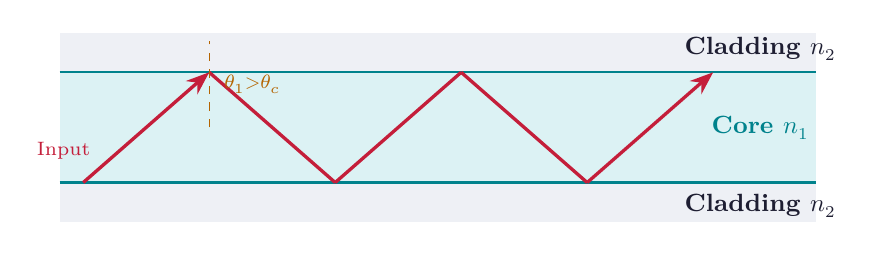
\begin{tikzpicture}[scale=1.0]
  % Cladding top and bottom
  \fill[hdrgray] (-0.1, 0.7) rectangle (9.5, 1.2);
  \fill[hdrgray] (-0.1, -1.2) rectangle (9.5, -0.7);
  % Core
  \fill[hdrteal] (-0.1, -0.7) rectangle (9.5, 0.7);
  % Labels
  \node[font=\small\bfseries\color{mydark}] at (8.8, 1.0) {Cladding $n_2$};
  \node[font=\small\bfseries\color{mydark}] at (8.8, -1.0) {Cladding $n_2$};
  \node[font=\small\bfseries\color{myteal}] at (8.8, 0.0) {Core $n_1$};
  % Boundaries
  \draw[thick, color=myteal] (-0.1, 0.7) -- (9.5, 0.7);
  \draw[thick, color=myteal] (-0.1, -0.7) -- (9.5, -0.7);
  % Ray path (zigzag using TIR)
  \draw[very thick, color=myred, -Stealth] (0.2, -0.7) -- (1.8, 0.7);
  \draw[very thick, color=myred] (1.8, 0.7) -- (3.4, -0.7);
  \draw[very thick, color=myred] (3.4, -0.7) -- (5.0, 0.7);
  \draw[very thick, color=myred] (5.0, 0.7) -- (6.6, -0.7);
  \draw[very thick, color=myred, -Stealth] (6.6, -0.7) -- (8.2, 0.7);
  % Angle annotations at first TIR point
  \draw[dashed, thin, color=myamber] (1.8, 0.0) -- (1.8, 1.1);
  \node[font=\scriptsize\color{myamber}] at (2.35, 0.55) {$\theta_1{>}\theta_c$};
  % Input ray label
  \node[font=\scriptsize\color{myred}] at (-0.05, -0.3) {Input};
\end{tikzpicture}
\end{tcolorbox}

% ===============================================================================
\section{Ray Model --- Acceptance Angle and Numerical Aperture}
% ===============================================================================

\begin{tcolorbox}[defbox, title={\textbf{Numerical Aperture (NA) and Acceptance Angle}}]
The \textbf{acceptance angle} $\theta_a$ (or half-cone angle) is the maximum angle at which light may enter the fiber end-face and still undergo TIR. The \textbf{Numerical Aperture (NA)} is a dimensionless measure of the light-gathering ability of the fiber: $\text{NA} = n_0 \sin\theta_a$ where $n_0$ is the refractive index of the medium at the input (usually air, $n_0 = 1$).
\end{tcolorbox}

\subsection{Derivation of NA}
Consider a ray entering the flat end of the fiber at angle $\theta_i$ (in air). By Snell's law at the end-face:
\[
\sin\theta_i = n_1 \sin\theta_r
\]
where $\theta_r$ is the refraction angle inside the core. For TIR at the core--cladding interface, the ray must strike that interface at an angle $\geq \theta_c$, meaning the complementary angle $\theta_r \leq (90^\circ - \theta_c)$. Using $\sin\theta_c = n_2/n_1$:

\begin{tcolorbox}[formulabox, title={\textbf{Numerical Aperture --- Complete Formula}}]
\[
\text{NA} = \sin\theta_a = \sqrt{n_1^2 - n_2^2}
\]
\[
\text{NA} = n_1\sqrt{2\Delta}, \qquad \Delta = \frac{n_1^2 - n_2^2}{2n_1^2} \approx \frac{n_1 - n_2}{n_1} \quad \text{(relative refractive index difference)}
\]
Acceptance angle: $\theta_a = \sin^{-1}(\text{NA})$ \quad (full acceptance cone = $2\theta_a$).
\end{tcolorbox}

\subsection{Meridional vs Skew Rays}
\begin{itemize}[leftmargin=*, itemsep=3pt]
  \item \textbf{Meridional rays:} Rays that pass through the fiber axis. Their path lies entirely in a plane containing the axis. They follow simple zigzag trajectories and are the easiest to analyze.
  \item \textbf{Skew rays:} Rays that do not pass through the fiber axis. They travel in a helical path around the axis. They have a larger acceptance angle than meridional rays and carry higher-order modes.
\end{itemize}

\begin{tcolorbox}[examplebox, title={\textbf{Worked Example: Calculate NA and Acceptance Angle}}]
Given: $n_1 = 1.48$, $n_2 = 1.46$. Find NA and $\theta_a$.
\[
\text{NA} = \sqrt{1.48^2 - 1.46^2} = \sqrt{2.1904 - 2.1316} = \sqrt{0.0588} \approx 0.2425
\]
\[
\theta_a = \sin^{-1}(0.2425) \approx 14.03^\circ, \qquad \Delta = \frac{1.48 - 1.46}{1.48} \approx 1.35\%
\]
\end{tcolorbox}

% ===============================================================================
\section{Wave Model --- Modes and V-Number}
% ===============================================================================

\begin{tcolorbox}[defbox, title={\textbf{Modes in an Optical Fiber}}]
A \textbf{mode} is a distinct spatial distribution (pattern) of the electromagnetic field that can propagate along the fiber without changing shape. Only certain discrete field patterns satisfy the boundary conditions at the core--cladding interface; these are the allowed or guided modes.
\end{tcolorbox}

\subsection{Normalized Frequency (V-Number)}
The \textbf{V-number} (also called the normalized frequency or normalized waveguide parameter) determines how many modes a fiber can support.

\begin{tcolorbox}[formulabox, title={\textbf{V-Number Formula}}]
\[
V = \frac{2\pi a}{\lambda}\,\text{NA} = \frac{2\pi a}{\lambda}\sqrt{n_1^2 - n_2^2} = \frac{2\pi a}{\lambda}\,n_1\sqrt{2\Delta}
\]
where $a$ = core radius, $\lambda$ = free-space wavelength of light.
\begin{itemize}[leftmargin=*, itemsep=2pt, topsep=4pt]
  \item $V < 2.405$ $\Rightarrow$ \textbf{single-mode} fiber (only the HE$_{11}$ fundamental mode propagates).
  \item $V \geq 2.405$ $\Rightarrow$ \textbf{multimode} fiber.
  \item Total number of modes (step-index): $M \approx \dfrac{V^2}{2}$.
  \item Total number of modes (graded-index, parabolic): $M \approx \dfrac{V^2}{4}$.
\end{itemize}
\end{tcolorbox}

\subsection{Cutoff Condition and Mode Designation}
Modes are designated HE$_{mn}$ or EH$_{mn}$ (hybrid modes), TE$_{0n}$, TM$_{0n}$. The fundamental mode HE$_{11}$ has no cutoff. The first higher-order mode TE$_{01}$ cuts off at $V = 2.405$ (first zero of Bessel function $J_0$).

\begin{tcolorbox}[examplebox, title={\textbf{Worked Example: V-Number and Mode Count}}]
Given: $a = 25\,\mu$m, $\lambda = 1300\,$nm, $n_1 = 1.48$, $n_2 = 1.46$.
\[
\text{NA} = 0.2425 \quad (\text{from previous example})
\]
\[
V = \frac{2\pi \times 25\times10^{-6}}{1300\times10^{-9}} \times 0.2425 = \frac{2\pi \times 25}{1.3} \times 0.2425 \approx 29.2
\]
Number of modes $M \approx V^2/2 \approx 426$. Since $V \gg 2.405$, this is a multimode fiber.
\end{tcolorbox}

% ===============================================================================
\section{Types of Optical Fibers}
% ===============================================================================

\begin{tcolorbox}[defbox, title={\textbf{Classification of Optical Fibers}}]
Optical fibers are classified by (a) \textbf{index profile} of the core --- step-index (SI) or graded-index (GI), and (b) \textbf{number of modes} --- single-mode (SM) or multimode (MM). The three main types are: Single-Mode Step-Index (SMF), Multimode Step-Index (MMSI), and Multimode Graded-Index (MMGI).
\end{tcolorbox}

\begin{tcolorbox}[tikzbox, title={Refractive Index Profiles and Ray Paths --- Three Fiber Types}]
\centering
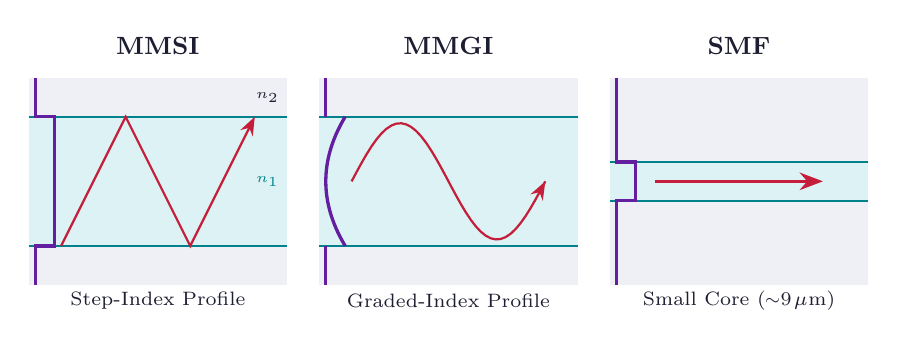
\begin{tikzpicture}[scale=0.82]
  % ── MMSI (left) ──────────────────────────────────────────────────────────
  \begin{scope}[xshift=0cm]
    \fill[hdrgray] (-0.5,-1.6) rectangle (3.5,-1.0);
    \fill[hdrteal] (-0.5,-1.0) rectangle (3.5, 1.0);
    \fill[hdrgray] (-0.5, 1.0) rectangle (3.5, 1.6);
    \draw[thick,color=myteal] (-0.5,1.0)--(3.5,1.0);
    \draw[thick,color=myteal] (-0.5,-1.0)--(3.5,-1.0);
    % zigzag ray
    \draw[thick,color=myred,-Stealth] (0,-1.0)--(1.0,1.0)--(2.0,-1.0)--(3.0,1.0);
    % index profile
    \draw[very thick,color=mypurple] (-0.4,-1.6)--(-0.4,-1.0)--(-0.1,-1.0)--(-0.1,1.0)--(-0.4,1.0)--(-0.4,1.6);
    \node[font=\small\bfseries\color{mydark},align=center] at (1.5,2.1) {MMSI};
    \node[font=\scriptsize\color{mydark}] at (1.5,-1.85) {Step-Index Profile};
    \node[font=\tiny\color{myteal}] at (3.2,0.0) {$n_1$};
    \node[font=\tiny\color{mydark}] at (3.2,1.3) {$n_2$};
  \end{scope}
  % ── MMGI (center) ─────────────────────────────────────────────────────────
  \begin{scope}[xshift=4.5cm]
    \fill[hdrgray] (-0.5,-1.6) rectangle (3.5,-1.0);
    \fill[hdrteal] (-0.5,-1.0) rectangle (3.5, 1.0);
    \fill[hdrgray] (-0.5, 1.0) rectangle (3.5, 1.6);
    \draw[thick,color=myteal] (-0.5,1.0)--(3.5,1.0);
    \draw[thick,color=myteal] (-0.5,-1.0)--(3.5,-1.0);
    % curved ray (sinusoidal)
    \draw[thick,color=myred,domain=0:3.0,samples=40,variable=\t]
      plot ({\t},{0.9*sin(360*\t/3.0)});
    \draw[-Stealth,thick,color=myred] (2.9,{0.9*sin(360*2.9/3.0)})--(3.0,{0.9*sin(360*3.0/3.0)});
    % parabolic index profile
    \draw[very thick,color=mypurple,domain=-1.0:1.0,samples=30,variable=\y]
      plot ({-0.4+0.3*\y*\y},{\y});
    \draw[very thick,color=mypurple] (-0.4,-1.6)--(-0.4,-1.0);
    \draw[very thick,color=mypurple] (-0.4,1.0)--(-0.4,1.6);
    \node[font=\small\bfseries\color{mydark},align=center] at (1.5,2.1) {MMGI};
    \node[font=\scriptsize\color{mydark}] at (1.5,-1.85) {Graded-Index Profile};
  \end{scope}
  % ── SMF (right) ───────────────────────────────────────────────────────────
  \begin{scope}[xshift=9.0cm]
    \fill[hdrgray] (-0.5,-1.6) rectangle (3.5,-0.3);
    \fill[hdrteal] (-0.5,-0.3) rectangle (3.5, 0.3);
    \fill[hdrgray] (-0.5, 0.3) rectangle (3.5, 1.6);
    \draw[thick,color=myteal] (-0.5,0.3)--(3.5,0.3);
    \draw[thick,color=myteal] (-0.5,-0.3)--(3.5,-0.3);
    % straight ray (single mode)
    \draw[very thick,color=myred,-Stealth] (0.2,0.0)--(2.8,0.0);
    % step profile (narrow)
    \draw[very thick,color=mypurple] (-0.4,-1.6)--(-0.4,-0.3)--(-0.1,-0.3)--(-0.1,0.3)--(-0.4,0.3)--(-0.4,1.6);
    \node[font=\small\bfseries\color{mydark},align=center] at (1.5,2.1) {SMF};
    \node[font=\scriptsize\color{mydark}] at (1.5,-1.85) {Small Core ($\sim$9\,$\mu$m)};
  \end{scope}
\end{tikzpicture}
\end{tcolorbox}

\subsection{Comparison Table --- SMF vs MMSI vs MMGI}

\par\noindent
{\renewcommand{\arraystretch}{1.55}
\begin{tabularx}{\linewidth}{|B{3.2cm}|Y|Y|Y|}
\hline
\textbf{Parameter} & \textbf{SMF} & \textbf{MMSI} & \textbf{MMGI} \\
\hline
Core diameter & $\sim$8--10\,$\mu$m & $\sim$50--200\,$\mu$m & $\sim$50--62.5\,$\mu$m \\
\hline
Cladding diameter & 125\,$\mu$m & 125--400\,$\mu$m & 125\,$\mu$m \\
\hline
Index profile & Step & Step & Parabolic ($\alpha \approx 2$) \\
\hline
V-number & $< 2.405$ & $\gg 2.405$ & $\gg 2.405$ \\
\hline
No.\ of modes & 1 (HE$_{11}$ only) & $\sim V^2/2$ (hundreds) & $\sim V^2/4$ \\
\hline
Bandwidth & Very high ($>$10\,GHz$\cdot$km) & Low ($\sim$10--25\,MHz$\cdot$km) & Medium ($\sim$400--2000\,MHz$\cdot$km) \\
\hline
Modal dispersion & None & High & Low (near-zero for $\alpha{=}2$) \\
\hline
NA & $\sim$0.1--0.12 & $\sim$0.2--0.5 & $\sim$0.2--0.3 \\
\hline
Coupling efficiency & Low (small core) & High & Medium \\
\hline
Light source & Laser only & LED or Laser & LED or Laser \\
\hline
Application & Long-haul, WDM & Short-haul, LAN & LAN, medium distance \\
\hline
\end{tabularx}}

% ===============================================================================
% QUICK REVISION PAGE
% ===============================================================================
\newpage
\begin{center}
  {\large\bfseries\color{myred} Quick Revision --- Module 1}\\[3pt]
  {\small\color{mydark} Light Propagation and Optical Fiber Fundamentals $|$ PE-EC801B}
\end{center}
\noindent{\color{myred}\rule{\linewidth}{1.2pt}}
\vspace{4pt}

\begin{tcolorbox}[formulabox, title={\textbf{Key Formulas at a Glance}}]
\renewcommand{\arraystretch}{1.35}
\begin{tabularx}{\linewidth}{B{5.0cm} X}
Snell's Law & $n_1 \sin\theta_1 = n_2 \sin\theta_2$ \\[4pt]
Critical angle & $\theta_c = \sin^{-1}(n_2/n_1)$ \quad ($n_1 > n_2$) \\[4pt]
Numerical Aperture & $\text{NA} = \sqrt{n_1^2 - n_2^2} = n_1\sqrt{2\Delta}$ \\[4pt]
Relative index diff.\ & $\Delta = (n_1 - n_2)/n_1$ (approx.\ for $n_1 \approx n_2$) \\[4pt]
V-number & $V = (2\pi a/\lambda)\,\text{NA}$ \\[4pt]
SMF condition & $V < 2.405$ \\[4pt]
Mode count (MMSI) & $M \approx V^2/2$ \\[4pt]
Mode count (MMGI) & $M \approx V^2/4$ \\[4pt]
Wave speed in medium & $v = c/n$; \quad $n = \sqrt{\epsilon_r}$ \\[4pt]
\end{tabularx}
\end{tcolorbox}

\begin{tcolorbox}[defbox, title={\textbf{One-Line Definitions}}]
\begin{itemize}[leftmargin=*, itemsep=2pt, topsep=0pt]
  \item \textbf{TIR:} Total Internal Reflection --- light stays in denser medium when $\theta_i \geq \theta_c$.
  \item \textbf{NA:} Numerical Aperture --- measure of light-gathering ability of the fiber.
  \item \textbf{V-number:} Normalized frequency parameter determining number of guided modes.
  \item \textbf{Meridional ray:} Ray passing through the fiber axis, zigzag path.
  \item \textbf{Skew ray:} Ray traveling in a helical path, does not pass through axis.
  \item \textbf{Mode:} Distinct stable field distribution pattern guided along the fiber.
  \item \textbf{SMF:} Single-mode fiber with $V < 2.405$; eliminates modal dispersion.
  \item \textbf{MMGI:} Multimode graded-index fiber; parabolic profile minimizes modal dispersion.
\end{itemize}
\end{tcolorbox}

\begin{tcolorbox}[exambox, title={\textbf{Frequently Asked / Viva Questions}}]
\begin{enumerate}[topsep=0pt, label=\textbf{Q\arabic*.}, itemsep=5pt]
  \item \Q{What is Total Internal Reflection and when does it occur?}
    TIR occurs when light travels from a denser medium ($n_1$) to a rarer medium ($n_2 < n_1$) and the angle of incidence exceeds the critical angle $\theta_c = \sin^{-1}(n_2/n_1)$. All incident light is reflected back; no energy enters medium 2.
  \item \Q{Why is the refractive index of the core greater than the cladding in an optical fiber?}
    TIR --- which is the guiding mechanism --- requires light to travel from a denser to rarer medium. Thus $n_1 > n_2$ is essential for guided propagation.
  \item \Q{Define Numerical Aperture (NA). What does a higher NA imply?}
    NA $= \sqrt{n_1^2 - n_2^2}$ is the sine of the maximum acceptance angle. Higher NA means the fiber accepts light over a wider cone but also supports more modes (greater modal dispersion).
  \item \Q{What is the V-number and what is its significance?}
    The V-number $= (2\pi a / \lambda)\,\text{NA}$ is the normalized frequency. It determines the number of guided modes. For $V < 2.405$, only one mode propagates (single-mode operation).
  \item \Q{Distinguish between meridional and skew rays.}
    Meridional rays pass through the fiber axis and travel in a plane containing it. Skew rays do not intersect the axis; they travel helically. Skew rays have a slightly larger effective acceptance angle.
  \item \Q{Why does a graded-index fiber have lower modal dispersion than step-index?}
    In MMGI, rays in the outer (faster) region travel longer paths but at higher speeds (lower $n$), while rays near the axis travel slower but shorter paths. This self-equalizing effect reduces pulse spreading.
  \item \Q{What is the cutoff condition for single-mode operation?}
    $V < 2.405$, where 2.405 is the first zero of the Bessel function $J_0$. Below this, only the fundamental HE$_{11}$ mode propagates.
  \item \Q{What is $\Delta$ (relative refractive index difference)?}
    $\Delta = (n_1 - n_2)/n_1 \approx (n_1^2 - n_2^2)/(2n_1^2)$. It is typically 0.1--2\% for communication fibers. Larger $\Delta$ means higher NA but also higher dispersion.
  \item \Q{How does the number of modes depend on V-number?}
    For step-index: $M \approx V^2/2$. For graded-index (parabolic): $M \approx V^2/4$. The graded profile halves the mode count for the same V-number.
  \item \Q{What are the dimensions of a standard SMF and MMSI fiber?}
    SMF: core $\sim$8--10\,$\mu$m, cladding 125\,$\mu$m. MMSI: core 50--200\,$\mu$m, cladding 125\,$\mu$m. MMGI: core 50--62.5\,$\mu$m, cladding 125\,$\mu$m.
  \item \Q{State the wave equation for the electric field in a dielectric medium.}
    $\nabla^2 \vec{E} = \mu\epsilon\, \partial^2\vec{E}/\partial t^2$. The speed of propagation is $v = 1/\sqrt{\mu\epsilon} = c/n$.
  \item \Q{What is the Poynting vector and what does it represent in fiber optics?}
    $\vec{S} = \vec{E} \times \vec{H}$ (W/m$^2$). It represents the direction and magnitude of electromagnetic power flow. In a fiber, it points along the fiber axis for guided modes.
\end{enumerate}
\end{tcolorbox}

\begin{tcolorbox}[tikzbox, title={Summary: Fiber Type Comparison at a Glance}]
\centering
{\renewcommand{\arraystretch}{1.45}
\begin{tabularx}{\linewidth}{|B{3.0cm}|Y|Y|Y|}
\hline
\textbf{Feature} & \textbf{SMF} & \textbf{MMSI} & \textbf{MMGI} \\
\hline
V-number & $< 2.405$ & Large & Large \\
\hline
Core dia.\ & 8--10\,$\mu$m & 50--200\,$\mu$m & 50--62.5\,$\mu$m \\
\hline
Dispersion & Lowest & Highest & Low \\
\hline
Bandwidth & Highest & Lowest & Medium \\
\hline
Source & Laser & LED/Laser & LED/Laser \\
\hline
Use case & Long haul & Short links & LAN/campus \\
\hline
\end{tabularx}}
\end{tcolorbox}

\end{document}
